\documentclass[12pt]{article} % use larger type; default would be 10pt


%%% PAGE DIMENSIONS
\usepackage[lmargin=.5in, rmargin=1.5in, marginpar=1.3in]{geometry} % to change the page dimensions (margins, etc.)
\geometry{letterpaper} % or letterpaper (US) or a5paper or....

\usepackage{graphicx} % support the \includegraphics command and options
\usepackage{CJKutf8}
\usepackage{makecell}
\usepackage{natbib}

% \usepackage[parfill]{parskip} % Activate to begin paragraphs with an empty line rather than an indent

%%% PACKAGES
\usepackage{setspace} % for changing line spacing
\usepackage{array} % for better arrays (eg matrices) in maths
\usepackage{paralist} % very flexible & customisable lists (eg. enumerate/itemize, etc.)
\usepackage{verbatim} % adds environment for commenting out blocks of text & for better verbatim
\usepackage{subfig} % make it possible to include more than one captioned figure/table in a single float
\usepackage[fleqn]{amsmath}
\usepackage{amsthm} % allows example and proof environment to be defined/used
\usepackage{amssymb}
\usepackage{todonotes}
\usepackage{nccmath}
\usepackage{hyperref}
\usepackage[ruled,vlined]{algorithm2e}
\usepackage{algorithmic}% http://ctan.org/pkg/algorithms

%Reference settings
\hypersetup{
    colorlinks=true,
    linkcolor=blue,
    filecolor=magenta,      
    urlcolor=cyan,
    pdftitle={Overleaf Example},
    pdfpagemode=FullScreen,
    }

%Algo definitions
\SetAlgorithmName{}{}{}
\SetKwRepeat{Do}{do}{while}%
\SetKw{KwBy}{by}

%%% HEADERS & FOOTERS
\usepackage{fancyhdr} % This should be set AFTER setting up the page geometry
\pagestyle{fancy} % options: empty , plain , fancy
\renewcommand{\headrulewidth}{0pt} % customise the layout...


\lhead{}\chead{}\rhead{}
\lfoot{}\cfoot{\thepage}\rfoot{}



%%% ToC (table of contents) APPEARANCE
\usepackage[nottoc,notlof,notlot]{tocbibind} % Put the bibliography in the ToC
\usepackage[titles,subfigure]{tocloft} % Alter the style of the Table of Contents


%%% SECTION COUNTER SETTINGS
\newcommand{\mysection}[2]{\setcounter{section}{#1}\section*{Chapter #1: #2}} % changes a "1" to "Chapter 1," and so on, and allows you to number the chapters manually if necessary. 


%%% COMPLETE AND INCOMPLETE COMMANDS
\newcommand{\incomplete}{$\square$}
\newcommand{\complete}{$\boxtimes$}
\usepackage{ marvosym }
\newcommand{\graded}{\Smiley}


%%% DEFINE EXAMPLE AND THEOREM ENVIRONMENTS
\theoremstyle{definition}
\newtheorem{example}{Example}
\newtheorem{lemma}{Lemma}
\newtheorem{theorem}{Theorem}
\newtheorem{definition}{Definition}
\newtheorem{notation}{Notation}
\newtheorem{prop}{Proposition}
\newtheorem{corollary}{Corollary}

%%MY MATH NOTATION%%
\newcommand{\A}{\mathcal{A}}
\newcommand{\E}{\mathbb{E}}
\newcommand{\F}{\mathcal{F}}
\newcommand{\Natural}{\mathbb{N}}
\newcommand{\Prob}{\mathbb{P}}
\newcommand{\Q}{\mathbb{Q}}
\newcommand{\ProbSpace}{(\Omega, \F. \mathbb{P})}
\newcommand{\Real}{\mathbb{R}}
\newcommand{\Shat}{\hat{S}}
\newcommand{\Time}{\mathcal{T}}
\newcommand{\Y}{\mathcal{Y}}

%%% END Article customizations

\title{Introduction to Gradient Descent}

\author{Jui Lu \\ Department of Money and Banking, National Chengchi Unversity}

%%% The "real" document content comes below...



\begin{document}

\maketitle

\subsection*{Brief Review of Convexity}

\noindent The materials is taken from

\begin{itemize}
	\item \cite{ahmadi15convex} lecture 7;
	\item \cite{audet2017derivative} chapter 2;
	\item \cite{boyd2004convex} chapter 2;
	\item \cite{schmidt18machine} lecture 3.
\end{itemize}

A convex optimization problem can be written in the form

$$
	\min_{x \in \Omega} f(x)
$$

\noindent where $f$ is a convex function and $\Omega$ is a convex set.

\begin{definition}[Convex Set]
	A set $\Omega$ is convex if and only if $\forall x, y \in \Omega$, and $\theta \in [0, 1]$, we have

	$$
		\theta x + (1 - \theta) y \in \Omega
	$$
\end{definition}

\begin{definition}[Convex Combination]
	A point $z \in \Real^n$ is a convex combination of the points in $\{x^{(1)}, \dots, x^{(m)}\} \subseteq \Real^n$ if there exists scalars $\theta^{(1)}, \dots, \theta^{(m)} \ge 0$ such that

	$$
		z = \sum_{i = 1}^m \theta^{(i)} x^{(i)} \quad \text{with } \sum_{i = 1}^m \theta^{(i)} = 1
	$$
\end{definition}

\begin{corollary}
	A set $\Omega$ is convex if convex combinations of points in the set are also in the set.
\end{corollary}

\begin{definition}[Convex Function]
	A function $f$ is convex if the area above the function, $\text{epi}(f)$, is a convex set, where

	$$
		\text{epi}(f) = \{[x, \alpha]^\intercal \in \Real^n \times \Real: \alpha \ge f(x) \}
	$$

	\noindent The set$\text{epi}(f)$ is called the epigraph of $f$. The equivalent statement is $\forall x, y \in \mathbf{dom}(f)$, and $\theta \in [0, 1]$,

	$$
		f(\theta x + (1 - \theta) y) \le \theta f(x) + (1 - \theta) f(y)
	$$
\end{definition}

\begin{theorem}[First-Order and Second-Order Convexity Condition]
	Suppose $f$ is twice-differentiable over an open domain. The the following are equivalent:
	
	\begin{enumerate}
		\item $f$ is convex;

		\item 1st-order condition:

		\begin{ceqn}
			\begin{equation}
				f(y) \ge f(x) + \nabla f(x)^\intercal (y - x) 
				\label{eq:convex function prop}
			\end{equation}
		\end{ceqn}

		\item 2nd-order condition: the Hessian matrix of $f$ is positive semidenite, i.e., the derivative is nondecreasing. 
	\end{enumerate}
\end{theorem}

\begin{proof}
	For the sake of simplicity, we only prove the result in case $n = 1$:

	\begin{itemize}
			\item $1. \Rightarrow 2.$: Suppose $f$ is convex and $x, y, \in \mathbf{dom}(f)$. Since $\mathbf{dom}(f)$ is convex, $\forall \theta \in (0, 1], (1 - \theta) x + \theta y = x + \theta (y - x) \in \mathbf{dom}(f)$. By convexity,
	
		\begin{ceqn}
			\begin{equation}
				f(x + \theta (y - x)) \le (1 - \theta) f(x) + \theta f(y)
				\label{eq: proof1 ineq1}
			\end{equation}
		\end{ceqn}
	
		Rearranging \eqref{eq: proof1 ineq1} yields
	
		\begin{ceqn}
			\begin{align*}
				f(y)
				&\ge f(x) + \frac{f(x + \theta (y - x)) - f(x)}{\theta} \\
				&= f(x) + (y - x) \times \frac{f(x + \theta (y - x)) - f(x)}{\theta (y - x)} \\
				&\rightarrow f(x) + (y - x) \times f'(x) \text{ as } \theta \rightarrow 0
			\end{align*}
		\end{ceqn}

		\item $1. \Leftarrow 2.$: Suppose $f$ statisfies \eqref{eq:convex function prop}. $\forall x, y \in \mathbf{dom}(f), x \ne y$ and $\theta \in [0, 1]$,  setting $z = \theta x + (1 - \theta) y$, we have

		$$
			f(x) \ge f(z) + f'(z) (x - z)
		$$

		and 

		$$
			f(y) \ge f(z) + f'(z) (y - z)
		$$

		 Multiplying the first inequality by $\theta$, the second by $1 - \theta$, and adding them yields

		\begin{ceqn}
			\begin{align*}
				\theta f(x) + (1 - \theta) f(y)
				&\ge \theta \big( f(z) + f'(z) (x - z) \big) + (1 - \theta)  \big( f(z) + f'(z) (y - z) \big) \\
				&= \theta \big( f(z) + f'(z) (1 - \theta) (x - y) \big) + (1 - \theta)  \big( f(z) + f'(z) \theta (x - y) \big) \\
				&= f(z)
			\end{align*}
		\end{ceqn}

		\item $2. \Rightarrow 3.$: $\forall x, y \in \mathbf{dom}(f), y > x$, we have

		$$
			f(y) \ge f(x) + f'(x) (y - x) \text{ and } f(x) \ge f(y) + f'(y) (x - y)
		$$

		hence

		\begin{ceqn}
			\begin{equation}
				f'(x) (y - x) \le f(y) - f(x) \le f'(y)(y - x)
				\label{eq:foc inequlity}
			\end{equation}
		\end{ceqn}

		Rearranging \eqref{eq:foc inequlity} obtains

		$$
			\frac{f'(y) - f'(x)}{y - x} \ge 0
		$$

		As we let $y \rightarrow x$, we get

		$$
			f''(x) \ge 0, \forall x \in \mathbf{dom}(f)
		$$

		\item $2. \Leftarrow 3.$: Suppose $f''(x) \ge 0, \forall x \in \mathbf{dom}(f)$. By the \href{https://math.stackexchange.com/questions/2522174/link-between-taylors-theorem-and-mean-value-theorem-question-about-the-frac}{mean value version of Taylors theorem}, $\forall x, y \in \mathbf{dom}(f), x < y$, $\exists z \in [x, y]$ s.t.

		$$
			f(y) = f(x) + f'(x) (y - x) + f''(z) (y - x)^2
		$$

		Since $f''(x) (y - x)^2 \ge 0$, we obtain

		$$
			f(y) \ge f(x) + f'(x) (y - x)
		$$
	\end{itemize}
\end{proof}


The inequality \eqref{eq:convex function prop} states that for a convex function, the first-order Taylor approximation is in fact a global underestimator of the function. Conversely, if the first-order Taylor approximation of a function is always a global underestimator of the function, then the function is convex.

\begin{figure}[h]
	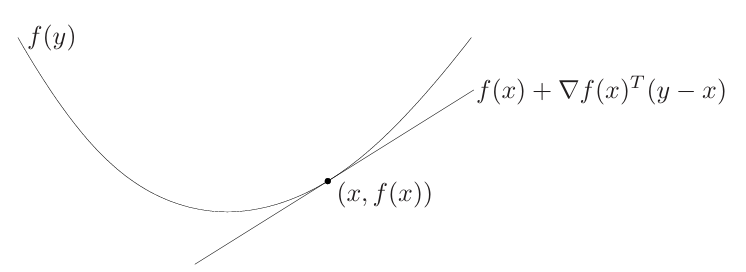
\includegraphics[width=13cm]{convex function prop.png}
	\centering
\end{figure}

\begin{example}[Univariate Convex Function]
	\hspace{1mm} \\
	\begin{itemize}
		\item Linear:

		$$
			f(x) = a + bx
		$$

		\item Quadratic:

		$$
			f(x) = a + bx + cx^2
		$$

		\item Exponential:

		$$
			f(x) = e^{ax}
		$$

		\item Negative logarithm

		$$
			f(x) = -\log x
		$$
	\end{itemize}
\end{example}

\vspace{1mm}

\begin{example}[Multivariate Convex Function]
	\hspace{1mm} \\
	\begin{itemize}
		\item Affine function:

		$$
			f(x) = a^\intercal x + b
		$$

		\item \color{red}\textbf{Any norm}\color{black}: Recall the definition of norm: Given a vector space $\mathbf{X}$ over a subfield $\mathbf{F}$ of the complex number $\mathbb{C}$, a norm on $\mathbf{X}$ is a real-valued function $\| \cdot \|: \mathbf{X} \rightarrow \Real$ with the following properties:

		\begin{enumerate}
			\item Subadditivity/Triangle inequality: $\|x + y\| \le \|x\| + \|y\|, \forall x, y \in \mathbf{X}$;
		
			\item Absolute homogeneity: $\|\alpha x\| = |\alpha| \|x\|, \forall x \in \mathbf{X}, \alpha \in \Real$;

			\item Positive definiteness/positiveness/Point-separating: if $\forall x \in \mathbf{X}, \|x\| = 0 \Rightarrow x = 0$.
		\end{enumerate}

		Applying properties 1. and 2. yields

		$$
			\| \theta x + (1 - \theta y)\| \le \| \theta x \| + \| (1 - \theta) y \| = \theta \|x\| + (1 - \theta) \|y\|, \forall x, y \in \mathbf{X}, \theta \in [0, 1]
		$$
	\end{itemize}
\end{example}

\noindent \color{red}\textbf{\underline{Note}}: In this handout, we set $\| \cdot \|$ to be the Euclidean norm, i.e., $\| x \| = \sqrt{\sum_{i = 1}^n x_i^2}$. \color{black} \\

\begin{definition}[Strict and Strong Convexity]
	A function $f:\Real^n \rightarrow \Real$ is 

	\begin{itemize}
		\item \textbf{strictly convex}, if $\forall x, y \in \mathbf{dom}(f),  x \ne y$, and $\theta \in (0, 1)$,

		$$
			f(\theta x + (1 - \theta) y) < \theta f(x) + (1 - \theta) f(y)
		$$

		\item   \textbf{$m$-strongly convex}, if $\exists m > 0$ s.t. $f(x) - m \|x\|^2$ is convex.
	\end{itemize}
\end{definition}

\begin{lemma}
	Strong convexity $\Rightarrow$ Strict convexity $\Rightarrow$ Convexity
\end{lemma}

\begin{proof}
	Since strict convexity $\Rightarrow$ convexity is obvious, we only prove strong convexity $\Rightarrow$ strict convexity. If a fucntion $f$ is strong convexity, $\forall x, y \in \mathbf{dom}(f),  x \ne y$, and $\theta \in (0, 1)$, we have

	$$
		f(\theta x + (1 - \theta y)) - m \| \theta x + (1 - \theta y)\|^2 \le \theta f(x) + (1 - \theta) f(y) - \theta m \|x\|^2 - (1 - \theta) m \| y \|^2
	$$

	Since $\| . \|^2$ is a strict convex function

	$$
		-  \theta m \|x\|^2 - (1 - \theta) m \| y \|^2 < -m \| \theta x + (1 - \theta y)\|^2
	$$

	and hence

	$$
		f(\theta x + (1 - \theta y)) - m \| \theta x + (1 - \theta y)\|^2 < \theta f(x) + (1 - \theta) f(y) - \theta m \|x\|^2 - (1 - \theta) m \| y \|^2
	$$
\end{proof}

Note that if $f$ is a $m$-strongly convex function, the function $g(x) = f(x) - m \| x \|^2$ is a convex function. By the first-order condition of convex function, we have

\begin{ceqn}
	\begin{align}
		&\, \, \quad g(y) \ge g(x) + \nabla g(x)^\intercal (y - x) \nonumber  \\
		&\Rightarrow f(y) - m \| y \|^2 \ge f(x) - m \| x \|^2 + (\nabla f(x) - 2 m x)^\intercal ( y - x) \nonumber \\
		&\Rightarrow f(y) \ge f(x) + \nabla f(x)^\intercal (y - x) + m \|y - x\|^2 
		\label{eq:strongly convex}
	\end{align}
\end{ceqn}

\subsection*{Gradient Descent Methods}

\noindent The materials is taken from

\begin{itemize}
	\item \cite{audet2017derivative} chapter 2;
	\item \cite{boyd2004convex} chapter 9;
	\item \cite{balakrishnan23convex} lecture 3;
	\item \cite{schmidt18machine} lecture 4;
	\item \cite{wang19convex} lecture 3.
\end{itemize}

Condiser an unconstrained optimization problem

$$
	\min_{x \in \Real^n} f(x)
$$

\noindent where $f: \Real^n \rightarrow \Real$ is a twice-differentiable convex  function. The algorithms described in this note produce a minimizing sequence $x_k, k = 1, \dots$, where

$$
	x_{k + 1} = x_k + t_k \Delta x_k
$$

\noindent and $t_k > 0$. We call $\Delta x_k$ a \textbf{descent direction} which is defined as follows:

\begin{definition}[Descent Direction]
	A direction $\Delta x_k \in \Real^n$ is said to be a descent direction of the function $f$ at the point $x_k \in \Real^n$ if and only if there exists a scalar $t_k \in (0, \bar{t}]$ such that

	$$
		f(x + t_k \Delta x_k) < f(x) \forall t_k \in (0, \bar{t}]
	$$
\end{definition}

The outline of descent method is written as follows

\begin{algorithm}
	\caption{General descent method}
  	\label{alg:descent method}
	\textbf{input: } $f, x \in \Real^n, k \leftarrow 0$ \\
	\textbf{do} \\
  	\begin{algorithmic}[1]
		\STATE Determine a descent direction $\Delta x_k$ \\
		\STATE \emph{Line search}: Choose a step size $t_k$ \\
		\STATE \emph{Update}: $x_{k + 1} = x_k + t_k \Delta x_k$ \\
		\STATE $k \leftarrow k + 1$
 	 \end{algorithmic}
	\textbf{until} (stopping criterion is satisfied) \\
\end{algorithm}

\newpage

The first step is searching the descent direction, from \eqref{eq:convex function prop} we know that $f(x_{k + 1}) = f(x_k +  t_k \Delta x_k) \ge f(x_k)$ implies

$$
	\nabla f(x)^\intercal t_k \Delta x_k \ge 0 
$$

\noindent Since $t_k \ge 0$,  the descent direction must satisfy

$$
	\nabla f(x)^\intercal \Delta x_k < 0
$$

Therefore, the natural choice of $\Delta x_k$ is $-\nabla f(x)$. This method is called \textbf{gradient descent method}. \\

The second question is how to choose the step size $t_k$? Here are som posibilities:

\begin{itemize}
	\item Fixed step size
	
	\item Exact line search

	\item Inexact line search
\end{itemize}


\subsubsection*{Fixed Step Size}

 We assume $\nabla f$ is $L$-Lipschitz i.e. $\exists L > 0$ s.t.

$$
	\| \nabla f(x) - \nabla f(y) \| \le L \|x - y \|, \forall x, y
$$

\begin{theorem}[Quadratic Upper Bound]
	$\nabla f$ is $L$-Lipschitz  implies

	\begin{enumerate}
		\item 

		\begin{ceqn}
			\begin{equation}
				(\nabla f(x) - \nabla f(y))^\intercal (x - y) \le L \| x - y \|^2, \forall x, y \in \mathbf{dom}(f)
				\label{eq:quadratic upper bound}
			\end{equation}
		\end{ceqn}
		
		\item If $\mathbf{dom}(f)$ is convex, \eqref{eq:quadratic upper bound} is equivalent to

		$$
			f(y) \le f(x) + f(x)^\intercal (y - x) + \frac{L}{2} \| y - x \|^2, \forall x, y \in \mathbf{dom}(f)
		$$
	\end{enumerate}
\end{theorem}

We state the descent lemma of gradient descent algorithm

\begin{lemma}[Descent Lemma]
	\label{lemma:descent lemma}
	If we run gradient descent for $k + 1$ iterations with a fixed step-size of $\frac{1}{L}$,  it will yield a solution $f(x_{k + 1})$ which satisfies

	$$
		f(x_{k + 1}) \le f(x_k) - \frac{1}{2L} \| \nabla f(x_k) \|^2
	$$
\end{lemma}

\begin{proof}
	The gradient descent update $x_{k + 1} = x_k - \frac{1}{L} \nabla f(x_k)$ gives

	$$
		x_{k + 1} - x_k = - \frac{1}{L} \nabla f(x_k)
	$$

	Since $\nabla f$ is $L$-Lipschitz, applying the quadratic bound property yields
	\begin{ceqn}
		\begin{align*}
			f(x_{k + 1})
			&\le f(x_k) + \nabla f(x_k)^\intercal (x_{k + 1} - x_k) + \frac{L}{2} \| x_{k + 1} - x_k \|^2 \\
			&=   f(x_k) - \nabla f(x_k)^\intercal \bigg( \frac{1}{L} \nabla f(x_k) \bigg) + \frac{L}{2} \Big\| \frac{1}{L} \nabla f(x_k) \Big\|^2 \\
			&=  f(x_k) - \frac{L}{2} \| \nabla f(x_k) \|^2
		\end{align*}
	\end{ceqn}
\end{proof}

According to Lemma \ref{lemma:descent lemma},   we start at some $f(x_0)$, and at each step we decrease f by at least $\frac{L}{2} \| \nabla f(x_k) \|^2$. So $\| \nabla f(x_k) \|^2$ must be going to zero \textbf{fast enough}.  Denote $x^*$ as an optimal solution for $f$, and $f^*$ as the optimal value. We have the following convergence guarantee for convex $L$-smooth function $f$:

\begin{theorem}
	\label{thm:convergence analysis fixed step}
	 Gradient descent with fxed step size $t \le \frac{1}{L}$ satisfies

	$$
		f(x_k) - f^* \le \frac{\|x_0 - x^*\|^2}{2tk}
	$$
\end{theorem}

\begin{proof}
	Since $f$ is a convex function, we have

	$$
		f(x_k) \le  f^* + \nabla f(x_k)^\intercal (x_k - x^*)
	$$

	Combined with Lemma \ref{lemma:descent lemma}, we have:

	\begin{ceqn}
		\begin{align*}
			f(x_{k + 1}) 
			&=  f(x_k) - \frac{t}{2} \| \nabla f(x_k) \|^2 \\
			&\le  f^* + \nabla f(x_k)^\intercal (x_k - x^*) - \frac{t}{2} \| \nabla f(x_k) \|^2 \\
			&=  f^* - \frac{1}{2t} \big( \| t \nabla f(x_k) \|^2 - 2t \nabla f(x_k)^\intercal (x_k - x^*) + \|x_k - x^*\|^2 - \|x_k - x^*\|^2 \big) \\
			&=  f^* - \frac{1}{2t} \big( \|t \nabla f(x_k) - (x_k - x^*)\|^2 - \|x_k - x^*\|^2 \big) \\
			&=  f^* - \frac{1}{2t} \big( \|x_{k +1} - x^* \|^2 - \|x_k - x^*\|^2 \big)
		\end{align*}
	\end{ceqn}

	Telescoping from $1$ to $k$, we can conclude the proof:

	\begin{ceqn}
		\begin{align*}
			& \, \, \quad  \sum_{i = 1}^k f(x_i) - k f^* \le  - \frac{1}{2t} \big( \|x_k - x^* \|^2 - \|x_0 - x^*\|^2 \big) \\
			&\Rightarrow \frac{1}{k} \sum_{i = 1}^k f(x_i) - f^*  \le \frac{\|x_0 - x^*\|^2}{2tk} \\
			&\Rightarrow f(x_k) - f^* \le \frac{\|x_0 - x^*\|^2}{2tk}
		\end{align*}
	\end{ceqn}
\end{proof}

\subsubsection*{Exact Line Search}
 The correct step size in many cases may depend on properties of the function that we don't know. In practice,  $L$ is usually expensive to compute, and $t_k = 1 / L$ is really small, hence \emph{we only need a step size this small in the worst case}. We consider solving the following 1D optimization
 problem to determine the best step-size

$$
	t_k = \min_{\tilde{t} > 0} f(x_k - \tilde{t} \nabla f(x_k))
$$

 Its often computationally cumbersome to solve this optimization problem exactly, so we resort to some approximation of this idea.

\subsubsection*{Inexact Line Search}

Most of practitioners use \textbf{inexact line search} - that is to say,  the step size is chosen to just reduce
$f$ \emph{enough}. The simplest inexact line search is \textbf{backtracking line search}. \\

\begin{algorithm}[h]
	\caption{Backtracking line search}
  	\label{alg:descent method}
	\textbf{input: } $x, \Delta x \in \Real^n, \alpha \in (0, 0.5), \beta \in (0, 1), \text{maxIter} \in \mathbb{N}, k \leftarrow 0, t \leftarrow 1$ \\
	\textbf{do while} ($k < \text{maxIter}$ and $f(x + t \Delta x) > f(x) + \alpha t \nabla f(x)^\intercal \Delta x$ ) \\
  	\begin{algorithmic}[1]
		\STATE $k \leftarrow k + 1$ \\
		\STATE $t \leftarrow \beta t$ \\
 	 \end{algorithmic}
\end{algorithm}

\newpage

Since $\Delta x$ is a descent direction,  $\nabla f(x)^\intercal \Delta x < 0$. For small enough $t$, we have

$$
	f(x + t \Delta x) \approx f(x) + t \nabla f(x)^\intercal \Delta x <  f(x) + \alpha t \nabla f(x)^\intercal \Delta x
$$

\begin{figure}[h]
	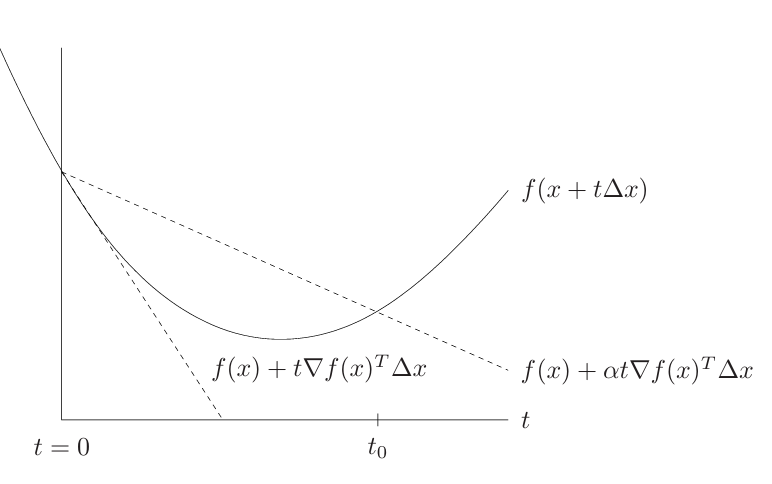
\includegraphics[width=13cm]{backtracking line search.png}
	\centering
\end{figure}

\begin{theorem}
	Suppose the function$f: \Real^n \rightarrow \Real$  is convex and differentiable, and $\nabla f$ is $L$-Lipschitz. Then if we run gradient descent for $k$ iterations with step size $t_k$ chosen using backtracking line search on each iteration $k$, it will yield a solution $f(x_k)$ which satisfies

	$$
		f(x_k) - f^* \le \frac{\| x_0 - x^* \|}{2t_\text{min}k}
	$$

	where $t_\text{min} = \min\{1, \beta / L\}$.
\end{theorem}

 Notice that if we choose $\beta$ to be large enough, the rate of convergence is very similar to what we got for gradient descent with fixed step size.

\subsubsection*{The Strongly Convex Case}

\begin{lemma}[A Gradient Bound under Smoothness]
	\label{lemma:gradient bound under smoothness}
	$$
		\| \nabla f(x) \|^2 \le 2L (f(x) - f^*)
	$$
\end{lemma}

\begin{proof}
	By quadratic upper bound, we have

	$$
		f^* \le f \bigg(x - \frac{1}{L} \nabla f(x) \bigg) \le f(x) - \frac{1}{L} \| \nabla f(x) \|^2 + \frac{1}{2L} \| \nabla f(x) \|^2 =  f(x) -  \frac{1}{2L} \| \nabla f(x) \|^2
	$$

	Rearranging above equation yields

	$$
		\| \nabla f(x) \|^2 \le 2L (f(x) - f^*)
	$$
\end{proof}

\begin{theorem}
	Let $f$ be a $m$-strongly convex and $L$-smooth function. Gradient descent with step size $t = 1 / L$, we have
	$$
		\| x_k - x^* \| \le \bigg(1 - \frac{2m}{L} \bigg)^k \| x_0 - x^* \|
	$$
\end{theorem}

\begin{proof}
	\begin{ceqn}
		\begin{align*}
			\| x_{k +1} - x^* \|^2 
			&= \| x_k - \nabla f(x) - x^* \|^2 \\
			&= \|x_k - x^*\|^2 - 2t \nabla f(x_k)^\intercal (x_k - x^*) + t^2 \| \nabla f(x_k) \|^2 \\
			&\le  \|x_k - x^*\|^2 - 2t (f(x_k) - f^* + m \| x_k - x^* \|^2) + t^2 \| \nabla f(x_k) \|^2 \quad \text{(By \eqref{eq:strongly convex})} \\
			&\le  \|x_k - x^*\|^2 - 2t (f(x_k) - f^* + m \| x_k - x^* \|^2) + 2 t^2 L (f(x_k) - f^*) \quad \text{(By Lemma \ref{lemma:gradient bound under smoothness})} \\
			&= \|x_k - x^*\|^2 - 2t m \| x_k - x^* \|^2 + 2t (tL - 1) (f(x_k) - f^*) \\
			&\le \|x_k - x^*\|^2 - 2t m \| x_k - x^* \|^2 \\
			&= \bigg(1 - \frac{2m}{L} \bigg) \| x_k - x^* \|
		\end{align*}
	\end{ceqn}
\end{proof}


\bibliographystyle{apalike}
\bibliography{reference}


\end{document}




